\documentclass[border=10pt]{standalone}

\usepackage{tikz}
\usepackage{tikzsymbols}
\usetikzlibrary{calc,patterns,shapes.geometric}

\def\centerarc[#1](#2)(#3:#4:#5){\draw[#1] ($(#2)+({#5*cos(#3)},{#5*sin(#3)})$) arc (#3:#4:#5);}

\begin{document}
	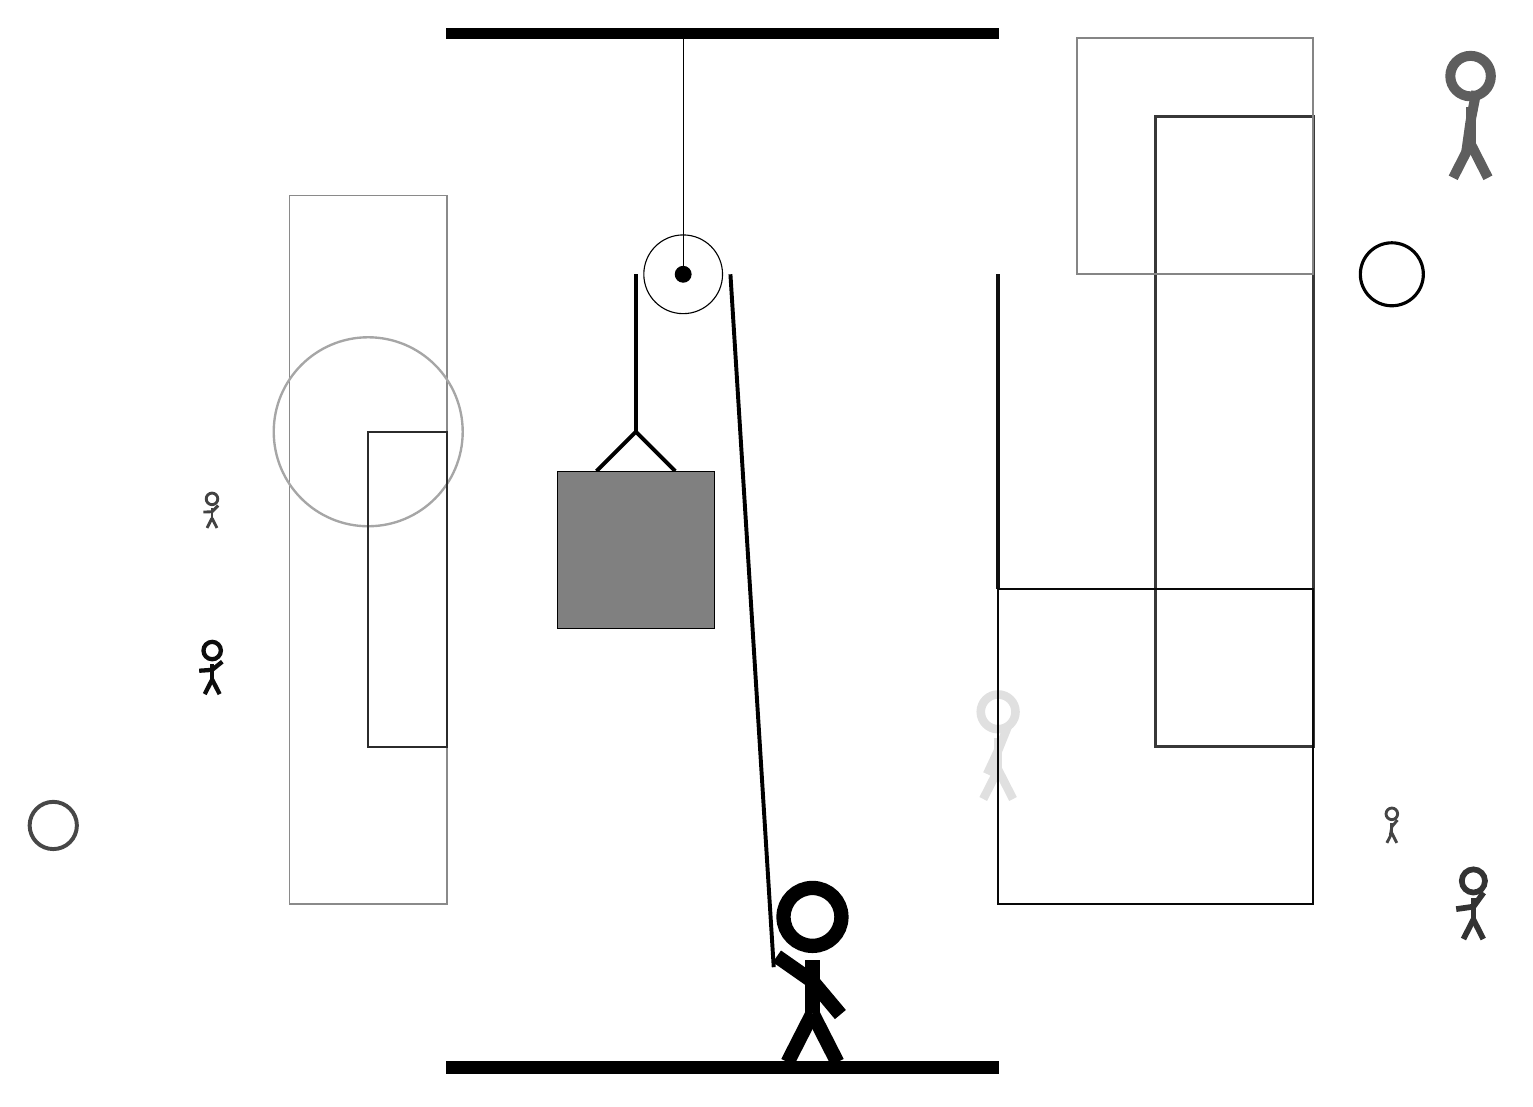
\begin{tikzpicture}
		%%%%% START %%%%%
		
		\draw[fill=black] (-2, 10) rectangle (5, 10.125);
		
		\draw (1, 7) circle (0.5);
		\draw[fill=black] (1, 7) circle (0.1);
		\draw (1, 10) -- (1, 7);
		
		\draw[line width=0.5mm] (-0.1, 4.5) -- (0.4, 5.0) -- (0.9, 4.5);
		\draw[fill=black!50] (-0.6, 4.5) rectangle (1.4, 2.5);
		
		\draw[line width=0.5mm] (0.4, 7) -- (0.4, 5.0);
		\centerarc[line width=0.5mm](1, 7)(0:180:0.6);
		\draw[line width=0.5mm](1.6, 7) -- (2.15, -1.8);
		
		\draw [line width=0.4mm, color=black!100](10, 7) circle (0.4);
		
		\node[line width=0.2mm, color=black!95] at (-5, 2) {\Strichmaxerl[3][4][39]};
		\draw[line width=0.4mm, color=black!78] (7, 1) rectangle (9, 9);
		\node[line width=0.4mm, color=black!12] at (5, 1) {\Strichmaxerl[6][65][68]};
		
		\draw[line width=0.5mm, color=black!94](5, 3) -- (5, 7);
		\node[line width=0.4mm, color=black!73] at (10, 0) {\Strichmaxerl[2][80][50]};
		
		\draw [line width=0.5mm, color=black!72](-7, 0) circle (0.3);
		
		\draw[line width=0.3mm, color=black!97] (5, -1) rectangle (9, 3);
		\node[line width=0.7mm, color=black!63] at (11, 9) {\Strichmaxerl[7][82][79]};
		
		\node[line width=0.6mm, color=black!80] at (11, -1) {\Strichmaxerl[4][8][54]};
		\draw[line width=0.2mm, color=black!46] (-4, 8) rectangle (-2, -1);
		\node[line width=0.5mm, color=black!74] at (-5, 4) {\Strichmaxerl[2][2][45]};
		\draw [line width=0.3mm, color=black!35](-3, 5) circle (1.2);
		
		\draw[line width=0.3mm, color=black!48] (6, 7) rectangle (9, 10);
		\draw[line width=0.2mm, color=black!83] (-2, 1) rectangle (-3, 5);
		
		\node at (2.6, -1.9) {\Strichmaxerl[10][-35][-50]};
		
		\draw[fill=black] (-2, -3) rectangle (5, -3.15);
		
		%%%%% END %%%%%
	\end{tikzpicture}
\end{document}